% =====================================================================
%  Prabhavit Gupta - two-page CV
%  Target: Customs Support Group - Customs AI Integration & Automation Engineer
%  Compile: tectonic main_CustomsSupport_AIEngineer.tex
%  Rules: STRICTLY TWO PAGES. No em-dashes. ASCII hyphens in dates.
% =====================================================================
\documentclass[a4paper,11pt]{article}

\usepackage[T1]{fontenc}
\usepackage[utf8]{inputenc}
\usepackage[top=1.3cm,bottom=1.3cm,left=1.5cm,right=1.5cm]{geometry}
\usepackage{titlesec}
\usepackage{enumitem}
\usepackage{hyperref}
\usepackage{xcolor}
\usepackage{graphicx}

\definecolor{accent}{HTML}{1F4E78}
\hypersetup{colorlinks=true, urlcolor=accent, linkcolor=accent}
\pagenumbering{arabic}
\setlength{\parindent}{0pt}

\titleformat{\section}{\large\bfseries\color{accent}}{}{0em}{}[\vspace{-0.6em}\rule{\textwidth}{0.8pt}]
\titlespacing{\section}{0pt}{7pt}{4pt}

\newcommand{\role}[4]{%
 \textbf{#1} \hfill \textbf{#2}\\[1pt]%
 \textit{#3} \hfill \textit{#4}\\[2pt]%
}
\setlist[itemize]{leftmargin=1.2em, itemsep=1.5pt, topsep=2pt, parsep=0pt}

\begin{document}

% ================= HEADER =================
\begin{minipage}[c]{0.80\textwidth}
 {\Huge\bfseries Prabhavit Gupta}\\[3pt]
 {\color{accent}\large Customs AI Integration \& Automation Engineer: Agentic Systems \& Document Pipelines}\\[6pt]
 {\footnotesize +39 351 610 7807 ~$\vert$~
 \href{mailto:prabhavitg@gmail.com}{prabhavitg@gmail.com} ~$\vert$~
 \href{https://www.linkedin.com/in/prabhavit/}{linkedin.com/in/prabhavit} ~$\vert$~
 \href{https://github.com/prab-gupta}{github.com/prab-gupta} ~$\vert$~
 Venice, Italy}
\end{minipage}\hfill
\begin{minipage}[c]{0.18\textwidth}
 \raggedleft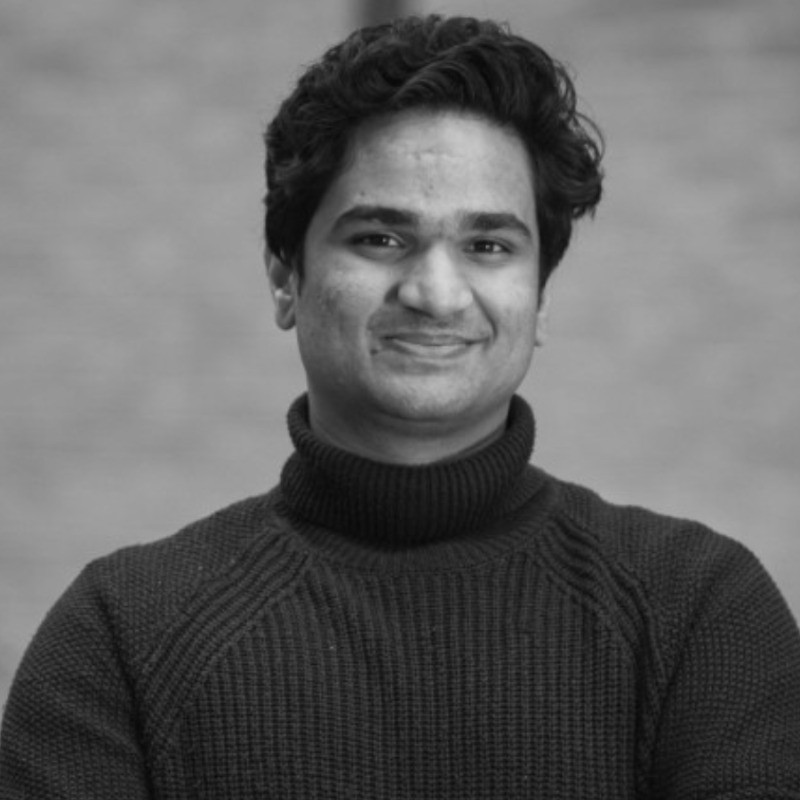
\includegraphics[width=2.0cm]{photo.jpg}
\end{minipage}
\vspace{-2pt}

% ================= SUMMARY =================
\section{Summary}
AI solutions and automation engineer with about three years of experience building and shipping LLM agent systems, automated document extraction pipelines, and customer API integrations. At FlowSpace I built an AI listing ingestion bot with human review that extracts structured entities from heterogeneous documents (PDFs, web pages, photos, spreadsheets) with 900+ listings drafted, and engineered AI support agents that answer queries against live platform data with confidence scoring and human escalation. Focused on reliable document understanding, explicit source data verification, and agentic workflows using n8n, Claude Code, Cursor, TypeScript, SQL, and working-level Python. Bachelor's in Philosophy, International Studies \& Economics. Italian EU long-term residence permit (permanent unrestricted right to work across the EU without sponsorship). Available immediately.

% ================= EXPERIENCE =================
\section{Experience}

\role{\href{https://flowspace.co}{FlowSpace.co}}{Mar 2024 - Aug 2026}{Lead Developer (Full-time, Freelance)}{London, UK (remote)}
\begin{itemize}
 \item Engineered an automated AI listing bot with human-in-the-loop review: ingests heterogeneous source files (PDF brochures, spreadsheets, images, web pages), extracts structured property and operational data via LLM prompts, audits outputs against original source data, and pushes approved entries to backend APIs. 900+ listings drafted.
 \item Implemented verification safeguards across document pipelines: audited generated fields against authoritative source data, enforced structured JSON output schemas, and verified final platform state via REST API readback.
 \item Built intelligent customer support agents utilizing tool use and function calling: queries live platform endpoints and escalates to human operators whenever model confidence falls below defined thresholds.
 \item Integrated multi-system platforms including OfficeRnD and Nexudus REST APIs for automated reservations, CRM lead capture, and outbound sales automations using n8n and webhooks.
 \item Led database schema mapping and platform migration to Next.js and Laravel, scaling user base from 2,000 to 4,500+ active users.
 \item \textit{Tools: Claude Code, n8n, Playwright, Postman, Laravel, TypeScript, Supabase, SQL, GitHub, Jira, Miro}
\end{itemize}

\role{\href{https://ultrastrategy.com}{UltraStrategy.com}}{Dec 2024 - May 2025}{Automation Developer (Collaborator)}{France}
\begin{itemize}
 \item Developed automated document extraction workflows using n8n and Eden AI to parse unstructured CV documents, extract candidate attributes, and populate relational schemas.
 \item \textit{Tools: n8n, Eden AI, REST APIs}
\end{itemize}

\role{\href{https://smarturlink.com/}{Urlink}}{Apr 2025 - Jul 2025}{Project Manager and AI-Assisted Developer (Freelance)}{Barcelona, Spain}
\begin{itemize}
 \item Designed and deployed AI-assisted platform architecture, user interfaces, and automated integration pipelines to meet customer specifications.
 \item \textit{Tools: GitHub, Netlify, Supabase, TypeScript}
\end{itemize}

\role{\href{https://www.qomodo.me/}{Qomodo}}{2024 - Jan 2025}{AI and Low-Code Developer (Collaborator)}{Milan, Italy}
\begin{itemize}
 \item Developed administrative dashboards and operational tooling for branch management, translating Figma designs into responsive interfaces.
\end{itemize}

\role{\href{https://get2germany.com}{Get2Germany.com}}{Jan 2024 - May 2024}{Lead Developer and Automation Specialist (Part-time)}{Berlin, Germany}
\begin{itemize}
 \item Built automated workflows and Google API integrations for user activity tracking, data consistency, and catalog discovery.
 \item \textit{Tools: n8n, Figma, Google APIs, relational databases}
\end{itemize}

\role{\href{https://clubee.com}{Clubee.com}}{Sep 2023 - Aug 2024}{Low-Code Developer and Quality Assurance (Full-time, Freelance)}{Foetz, Luxembourg}
\begin{itemize}
 \item Integrated Clubee REST APIs across web applications, conducted automated and manual QA testing on new features, and developed federation administration tools.
 \item \textit{Tools: Figma, GitHub, Postman, REST APIs}
\end{itemize}

\role{\href{https://tractionboard.co}{Tractionboard.co}}{Aug 2023 - Oct 2023}{Low-Code Developer (Internship)}{Utrecht, Netherlands}
\begin{itemize}
 \item Integrated OpenAI API and SendGrid communication pipelines, developed responsive web interfaces, and configured analytics tracking.
 \item \textit{Tools: OpenAI API, Sendgrid, Figma}
\end{itemize}

% ================= EDUCATION =================
\section{Education}
\role{Ca' Foscari University of Venice}{Oct 2020 - Jun 2024}{Bachelor's in Philosophy, International Studies \& Economics, Minor in Entrepreneurship}{Venice, Italy}

% ================= CERTIFICATIONS =================
\section{Certifications}
Microsoft Copilot Studio Agent Academy \textbullet\ Microsoft: Introduction to building AI agents \textbullet\ Microsoft Power Automate \textbullet\ Tray.AI Build Practitioner (Sep 2024) \textbullet\ Tray.AI Build Foundations

% ================= ADDITIONAL INFORMATION =================
\section{Additional Information}
\begin{itemize}
 \item \textbf{Work authorization:} European Long Term Residence Permit (Italy), permanent unrestricted right to work across the EU without sponsorship. Available immediately.
 \item \textbf{Languages:} Hindi (native), English (professional), Italian (beginner).
\end{itemize}

% ================= CORE SKILLS =================
\section{Core Skills}
\begin{itemize}
 \item \textbf{AI \& Document Automation:} LLM agents, document parsing (PDF, tables, OCR), prompt engineering, structured JSON extraction, human-in-the-loop workflows, confidence scoring, Claude Code, Cursor
 \item \textbf{System Integration \& Data:} REST APIs, webhooks, OAuth, n8n, SQL, schema design, Supabase, PostgreSQL, Postman, Google APIs
 \item \textbf{Engineering \& Quality:} TypeScript, JavaScript, Node.js, Python (working level), Laravel, Playwright, Git, CI/CD basics, Jira
 \item \textbf{Solution Architecture:} Business process analysis, document validation rules, verification harnesses, technical documentation
\end{itemize}

\end{document}
